%!TEX root =  ../main.tex

\mychapters{Conics}{conics}{\chapdir/pics/NM_12-06-06_0576_(7175101925)}

Rotated, Eccentricity

\newpage
\chapterminitoc

\newpage
\invisiblesection{Introduction to Conics}
\marginlessinput{\chapdir/DD01p}
%Extrapolate to infinite plane intersecting infinite (double) cone.  Discover circles, ellipses, parabola, hyperbola and record angles relative to cone.  Graph $x^2+y^2=1$, $x^2/4+y^2=1$, $x+y^2=1$, $x^2-y^2=1$.
\newpage
%!TEX root =  ../main.tex

\subsection{3D Geometry}
For nearly 3,000 years, mathematicians have been interested in shapes called
conic sections.  Why?  What are they?  Surprisingly, they are the means to answer some
very basic problems, like doubling the size of a cube, or why it is almost impossible to make
a square with the same area as a circle.  While the Ancient Greek geometers were interested
in such problems, it is far easier to consider them in light of analytic geometry, where we 
lay down the Cartesian plane, and place shapes in it, analyzing the algebra of their equations.

\marginfig[-0.5in]{\chapdir/pics/ConicSections_ajl.png}{The conic sections.}
The problems you worked in the lab were examples of three out of the four conic sections.
Why are they called such?  It is easy to model a cone intersecting a plane.  If we
imagine the cone as an idealized version of itself, it extends both up and down, forever
in two directions.  The plane of intersection is also the infinite plane of geometry, a flat
sheet that extends forever.

If the line through the middle of the cone intersects the plane at $90^\circ$ precisely
(what mathematicians call \textbf{normal} to the plane), then the shape on the plane will
be incredibly symmetrical, a \textbf{circle}.  Any slight variance in that angle will produce a
distorted circle, what is ordinarily called an `oval', but in mathematical parlance, an
\textbf{ellipse}. If we continue to tilt the plane, the ellipse will widen and widen.  As we
achieve an angle parallel to the side of the cone, the shape is our old friend, the 
\textbf{parabola}.  Any angle past that will result in intersecting both parts of the cone,
a shape known as a \textbf{hyperbola}.

\subsection{Graphing form}
\subsubsection{Circles}
Drawing circles is very easy and so is the algebra equation underlying them.  With a center
at $(h,k)$ and radius $r$, they can be quickly graphed, even by hand.

\marginfig[-0.5in]{\chapdir/pics/Conic_sections.png}{The angle of intersection of the plane 
and the cone may be plainly seen in the projection.}
\begin{derivation}{Equation of a Circle}
\label{eq:circle}
\begin{equation}
(x-h)^2+(y-k)^2=r^2
\end{equation}
\end{derivation}

\subsubsection{Ellipses}
We could imagine an straight-forward algebra manipulation which mirrors the geometric
manipulation from circles to ellipses: begin with Eq.~\ref{eq:circle}.  Now divide both sides 
by $r^2$:
$$
\frac{(x-h)^2}{r^2} + \frac{(y-h)^2}{r^2} = 1
$$
If we consider that the two radii represented in the denominators might be different 
(perhaps we might relabel them as $r_1^2$
and $r_2^2$), then we are very close to the graphing form of the equations for ellipses, and
we have a visual parallel: an ellipse is a circle with different radii for the $x$ and $y$!

\begin{derivation}{Equations of Ellipses}
\begin{equation}
\label{eq:ellipses}
\left(\frac{x-h}{a}\right)^2 + \left(\frac{y-k}{b}\right)^2 = 1 \quad \text{or} \quad \left(\frac{x-h}{b}\right)^2 + \left(\frac{y-k}{a}\right)^2 = 1
\end{equation}
\end{derivation}
By convention, we call whichever radii is bigger $a$, hence the two different forms.  (It will become
clearer in §DD.04 why.)

\subsubsection{Parabola}
You have done a lot of work with parabolas over the years, and the vertex form of Algebra II
requires very little manipulation to adapt to our purposes here (i.e. $y=a(x-h)^2+k$).  The only
caveats are that we like to keep the unit $(y-k)$ together, and that $a$ is four times the focal
length, conventionally called $p$.  Also, there are parabolas that open up-down, as well
as those that open left-right, as we saw in §3.3

\begin{derivation}{Equations of Parabolas}
\begin{equation}
(y-k) = 4p(x-h)^2 \quad  \text{or} \quad (x-h) = 4p (y-k)^2
\end{equation}
\end{derivation}

\subsection{Hyperbolas}
\marginfig[-1in]{\chapdir/pics/Drini-conjugatehyperbolas.png}{Hyperbolas can be horizontally or vertically oriented.}
Hyperbolas are very likely the least familiar to you of any of these objects.  Of course, 
$y=\frac{1}{x}$ is a hyperbola, but that can be hard to see, unless you turn your head
$45^\circ$ to the left!  If you look at the hyperbola $x^2-y^2=1$, some of the standard 
features are apparent.  There are two asymptotes, in this case, at $y=\pm x$.  They 
go through the center of the graph (the origin), which is not part of the graph.  These
same two asymptotes would be the same ones for the graph of $y^2-x^2=1$, only
one opens left-right, while the other one is oriented up-down.

\begin{derivation}{Equations of Hyperbolas}
\begin{equation}
\left(\frac{x-h}{a}\right)^2 - \left(\frac{y-k}{b}\right)^2 = 1
\quad \text{or} \quad
\left(\frac{y-k}{a}\right)^2 - \left(\frac{x-h}{b}\right)^2 = 1
\end{equation}
\end{derivation}

Practically speaking, graphing from the equation is a multi-step process
\begin{enumerate}
\item Begin at the center $(h,k)$.
\item Whichever variable is underneath $x$ (either $a$ or $b$), proceed that distance right and left from the center.
\item Whichever variable is underneath $y$ (either $b$ or $a$), proceed that distance up and down from the center.  
\item The preceeding dimensions are needed to draw the asymptotes, which either have slopes of $\pm\frac{b}{a}$ or $\pm\frac{a}{b}$.
\end{enumerate}

\marginfig[0in]{\chapdir/pics/Giperbola-koord.png}{A horizontal hyperbola centered at the origin.}

\newpage
\subsection{Exercises}
in Kuta


\newpage
\section{Algebra Manipulations}
\noindent\makebox[\textwidth]{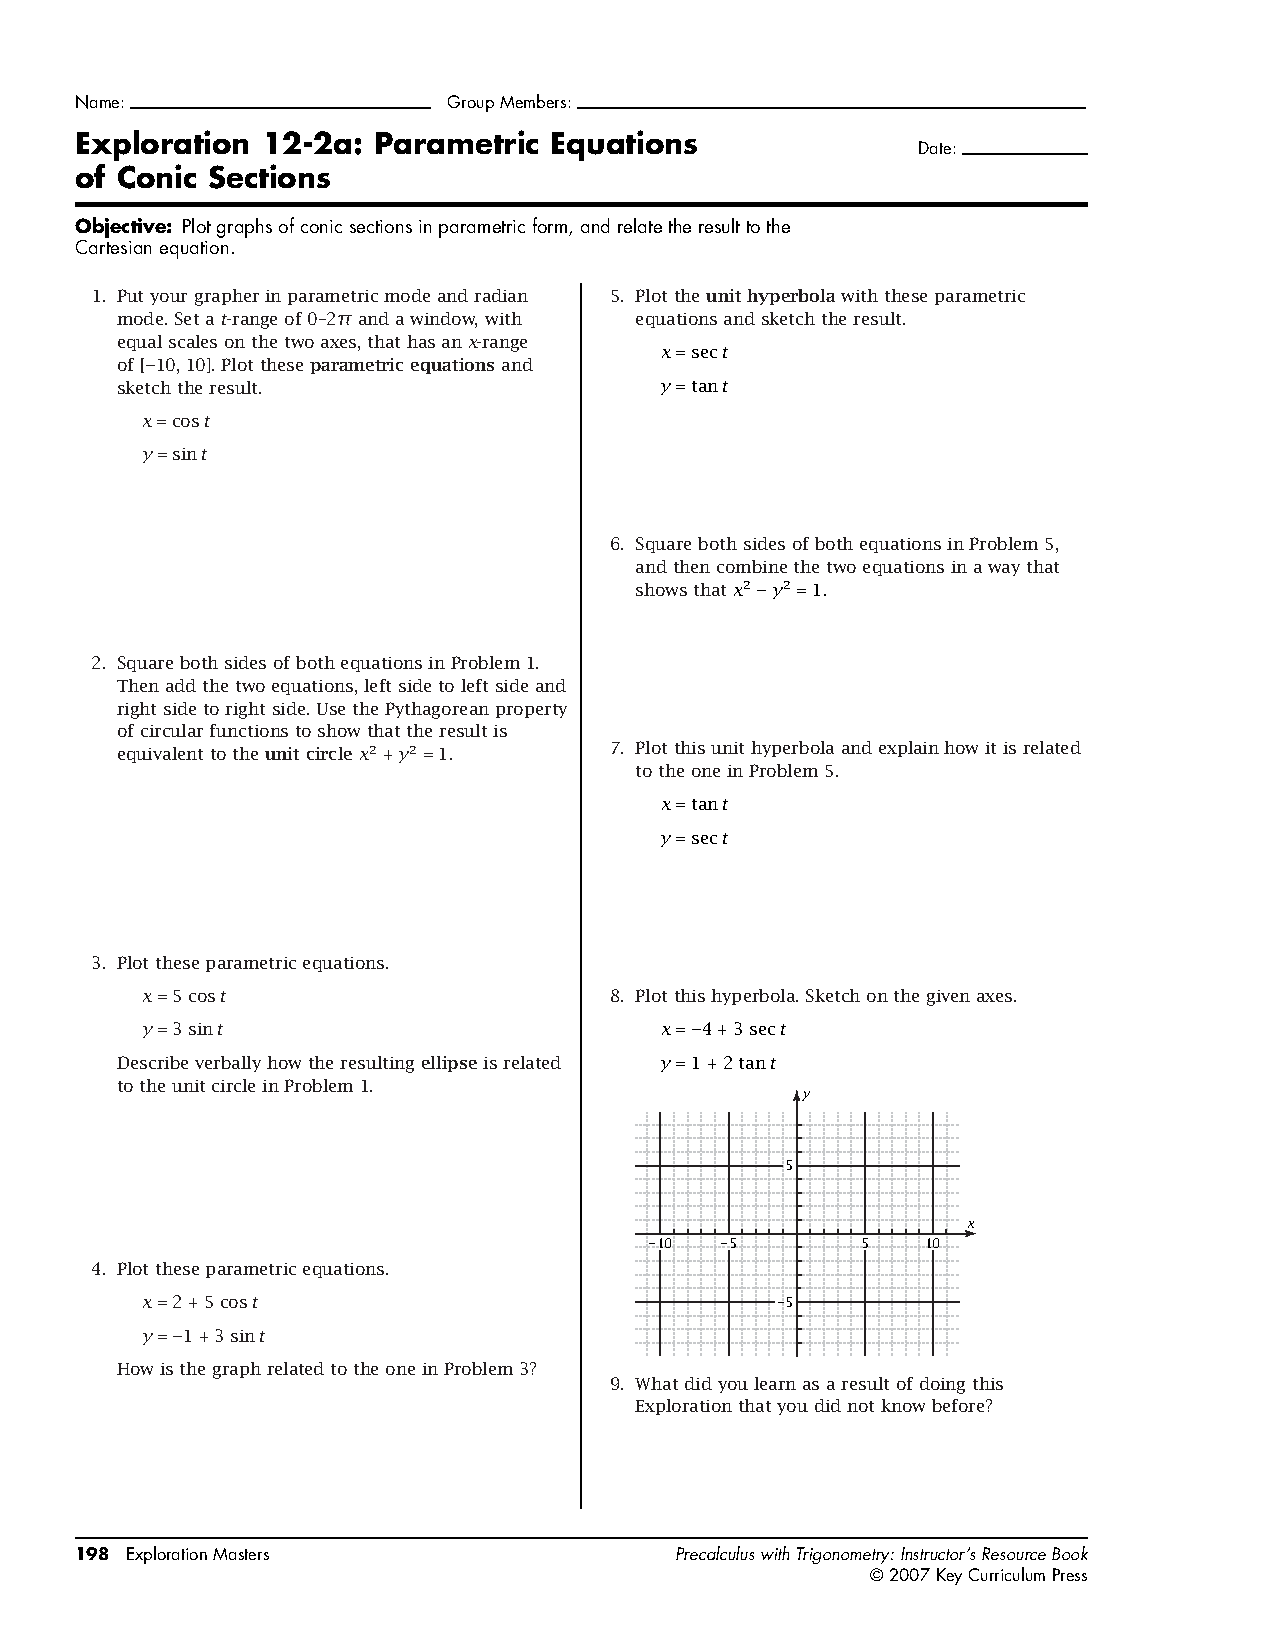
\includegraphics[width=\paperwidth]{chDD/DD02p.pdf}}
\subsection{Parametric Forms}
Conic sections lend themselves incredibly well to a variety of forms.  We saw in the last section that the Cartesian form
\subsection{Polar Forms}
\subsection{Algebra General Form}
\subsection{Using a Calculator}
\subsection{Discriminant}
\subsection{Completing the Square}
\subsection{Cartesian Forms}

\newpage
\section{Rotated Conics}
\subsection{Rotated Polar Conics}
\subsection{Cartesian Rotation Equations}
\subsection{Parametric Rotation by Matrix}

\newpage
\section{Eccentricity}
\subsection{Range of Eccentricity}
\subsection{Foci}
\subsection{Directrices}
\subsection{Distance Formulae}

\newpage
\section{3D Conics}
\noindent\makebox[\textwidth]{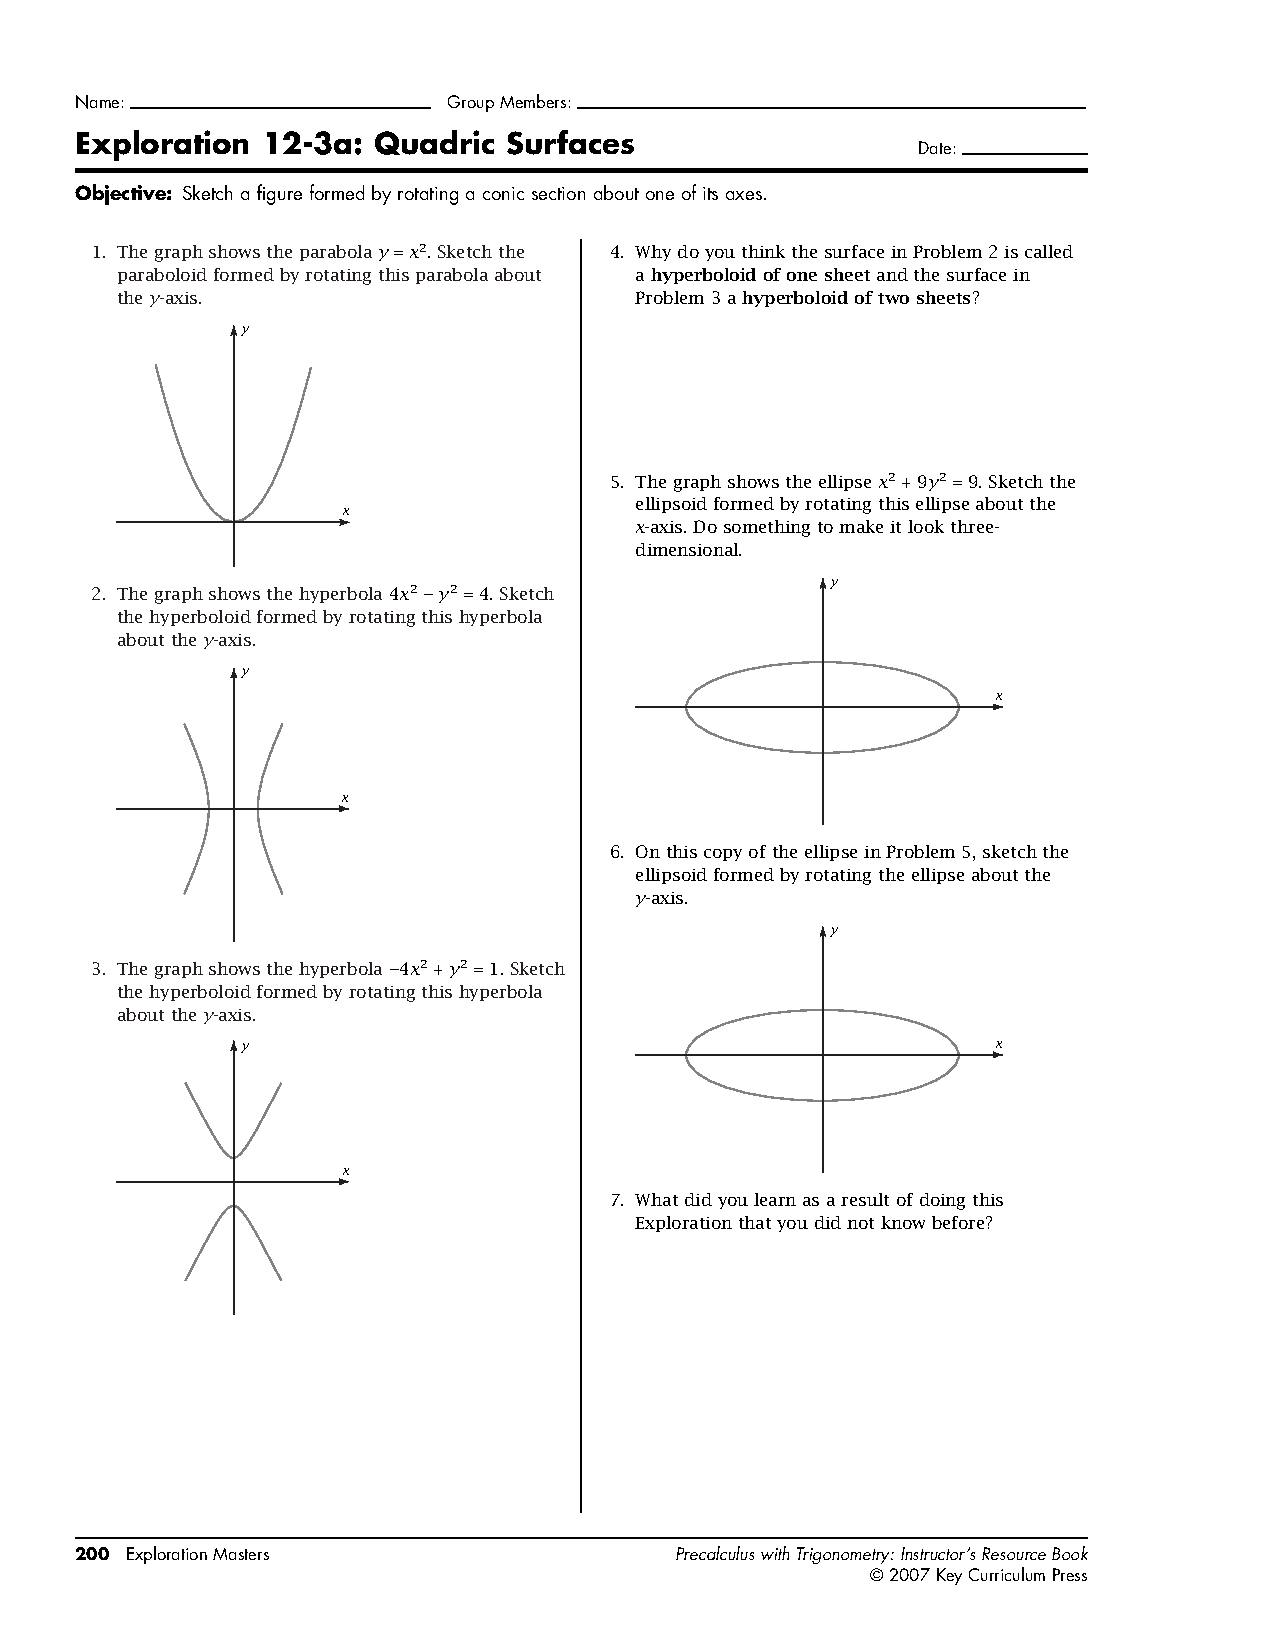
\includegraphics[width=\paperwidth]{chDD/DD05p.pdf}}
\subsection{2.5D}
\subsection{$x, y, z$}
\subsection{$r, \theta, z$}
\subsection{$\rho, \phi, \theta$}

\section{Chapter Review}